\documentclass[tikz,border=10pt]{standalone}
\usepackage{amsmath,amssymb}
\usetikzlibrary{arrows.meta, calc}

\begin{document}
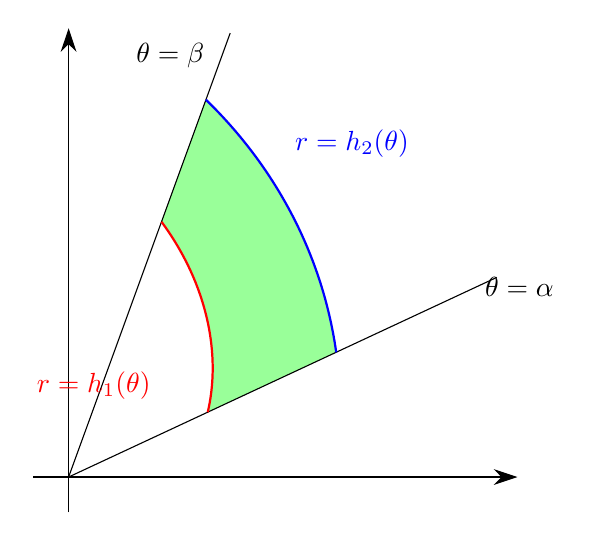
\begin{tikzpicture}[
    scale=1.5,
    >={Stealth[length=3mm, width=2mm]}
]

% Define angles (in degrees)
\def\alphaAngle{25}
\def\betaAngle{70}

% --- Shaded region (green fill) ---
% Create a path that goes along h1 from alpha to beta, then along h2 from beta to alpha
\fill[green!40]
    plot[smooth, domain=\alphaAngle:\betaAngle, samples=50]
        ({\x}:{1.3 + 0.8*(\x-\alphaAngle)/(\betaAngle-\alphaAngle) + 0.2*((\x-\alphaAngle)/(\betaAngle-\alphaAngle))^2})
    --
    plot[smooth, domain=\betaAngle:\alphaAngle, samples=50]
        ({\x}:{2.5 + 0.6*(\x-\alphaAngle)/(\betaAngle-\alphaAngle) + 0.3*((\x-\alphaAngle)/(\betaAngle-\alphaAngle))^2})
    -- cycle;

% --- Coordinate axes ---
\draw[->] (-0.3,0) -- (3.8,0);
\draw[->] (0,-0.3) -- (0,3.8);

% --- Rays for theta = alpha and theta = beta ---
\draw (0,0) -- ({\alphaAngle}:4.0);
\draw (0,0) -- ({\betaAngle}:4.0);

% --- Inner curve r = h1(theta) (red) ---
\draw[red, thick]
    plot[smooth, domain=\alphaAngle:\betaAngle, samples=50]
        ({\x}:{1.3 + 0.8*(\x-\alphaAngle)/(\betaAngle-\alphaAngle) + 0.2*((\x-\alphaAngle)/(\betaAngle-\alphaAngle))^2});

% --- Outer curve r = h2(theta) (blue) ---
\draw[blue, thick]
    plot[smooth, domain=\alphaAngle:\betaAngle, samples=50]
        ({\x}:{2.5 + 0.6*(\x-\alphaAngle)/(\betaAngle-\alphaAngle) + 0.3*((\x-\alphaAngle)/(\betaAngle-\alphaAngle))^2});

% --- Labels ---
% theta = beta label (upper ray) - positioned above the ray
\node[anchor=south east] at ({\betaAngle}:3.6) {$\theta = \beta$};

% theta = alpha label (lower ray) - positioned to the right
\node[anchor=west] at ({\alphaAngle}:3.8) {$\theta = \alpha$};

% r = h1(theta) label (red, inside the region near inner curve)
\node[red, anchor=east] at ({45}:{1.1}) {$r = h_1(\theta)$};

% r = h2(theta) label (blue, outside near outer curve)
\node[blue, anchor=south west] at ({55}:{3.2}) {$r = h_2(\theta)$};

\end{tikzpicture}
\end{document}
